\documentclass[11pt]{article}
\usepackage[margin=0.75in,top=0.7in,bottom=0.7in]{geometry}
\usepackage{graphicx,amsmath,amssymb,booktabs,array,xcolor}
\usepackage{fancyhdr,titlesec,enumitem,caption,float}
\usepackage[T1]{fontenc}
\usepackage[colorlinks=true,linkcolor=blue,urlcolor=blue,citecolor=blue]{hyperref}

\captionsetup{font=small,labelfont=bf}
\setlist{itemsep=1pt,topsep=2pt,parsep=0pt}
\titlespacing*{\section}{0pt}{9pt}{4pt}
\titlespacing*{\subsection}{0pt}{7pt}{3pt}
\pagestyle{fancy}\fancyhf{}
\lhead{}\rhead{\small SERF-MAD Integration -- SR}
\cfoot{\small\thepage}
\renewcommand{\headrulewidth}{0.4pt}

\newcommand{\band}{\begin{center}\rule{\linewidth}{0.8pt}\end{center}}
\newcommand{\nT}{\,nT}\newcommand{\pT}{\,pT}\newcommand{\fT}{\,fT}

% Provenance markers. Every number in this report carries one.
\newcommand{\meas}{\textcolor{blue!55!black}{\footnotesize[M]}}
\newcommand{\sig}{\textcolor{violet!70!black}{\footnotesize[S]}}
\newcommand{\assm}{\textcolor{red!65!black}{\footnotesize[A]}}
\newcommand{\lit}{\textcolor{teal!70!black}{\footnotesize[L]}}

\begin{document}
\thispagestyle{fancy}
\band
\begin{center}
{\large\bfseries Structural and Material Integration of a SERF MEMS\\[2pt]
Magnetometer Payload in an Autonomous Underwater Vehicle}\\[8pt]
{\normalsize Towed-Body Mechanics, Magnetic Cleanliness, and a Geometry-Derived
Rejection Limit}\\[10pt]
{\small Scientific Report --- Companion to the SERF-MAD Feasibility Study}\\[8pt]
{\small 16 August 2026}
\end{center}
\band
\vspace{-0.2cm}

\begin{center}\small
\fbox{\parbox{0.96\linewidth}{\centering
\textbf{Provenance convention.} Every quantitative claim is marked:
\meas~measured and cited \quad
\lit~literature closed form evaluated here \quad
\sig~simulated \quad
\assm~engineering assumption.\\
Unmarked numbers are restated from the parent feasibility study.}}
\end{center}
\vspace{-0.15cm}

\section*{Executive Summary}
\noindent The parent feasibility study \cite{srreport} established that a
ruggedised SERF MEMS magnetometer is a physically credible AUV magnetic anomaly
detection payload, and that its feasibility is governed not by sensor
sensitivity --- which exceeds requirement by five orders of magnitude
\cite{griffith2010,oehler2024} --- but by ambient-field control and platform
magnetic cleanliness. It derived a residual-field requirement of
$\leq0.94\nT$ ($94$~dB of suppression) from the Cross-Axis Projection Error
\cite{borna2022}, and demonstrated by sensitivity analysis that the system is
clutter-limited: the elasticity of detection range with respect to sensor noise
is exactly zero, while clutter magnitude, rejection ratio and gradiometer
baseline all register near $0.2$.

That study deliberately placed hydrodynamic design out of scope, represented
passive shielding as a scalar multiplier, and represented platform self-field as
a parametric common-mode rejection ratio rather than deriving it from vehicle
geometry and materials. This report addresses those three gaps. It executes
Recommendation~3 of the parent study --- replace the parametric rejection ratio
with a geometry-based vehicle magnetic model --- and reports three findings.

\begin{enumerate}[leftmargin=1.5em]
\item \textbf{Gradiometric rejection of the platform is limited by geometry, not
by channel matching.} A two-cell gradiometer rejects a \emph{uniform} field to
the limit set by gain and axis matching, and for the $0.1\%$ matching of
requirement R-09 that is $60$~dB. The vehicle's own sources are not uniform:
they sit metres from the baseline, so their field has a genuine gradient across
it which no amount of matching removes. Deriving the rejection from component
placement gives $5.5$~dB at a $2$~m standoff\sig, not $60$~dB. Reaching $60$~dB
against a near-field source by standoff alone would require a $1500$~m boom.
The parent study anticipates this mechanism qualitatively in its test X-07
discussion; this report quantifies it.

\item \textbf{Magnetic cleanliness is dominated by remanence, and remanence is a
build-time property.} Induced magnetisation scales with the ambient field and
therefore vanishes inside a shield; remanent magnetisation does not. Substituting
the material of an otherwise identical fastener set changes the field at the
sensor by more than six orders of magnitude, from $999.9\pT$ for cold-worked
316L to $4.6\times10^{-4}\pT$ for CFRP\sig. The ranking is robust; the
magnitudes rest on assumed remanence values and are flagged accordingly.

\item \textbf{The passive shield closes the $94$~dB budget only if it is annealed
in its final form.} The $0.94\nT$ requirement implies $53{,}191\times$ total
suppression, hence a $532\times$ passive stage against the study's $100\times$
active stage\lit. An annealed mu-metal cylinder of $5$~cm diameter and $1$~mm
wall delivers $1119\times$\lit. The same alloy formed from foil and not
re-annealed delivers $93\times$ and fails the requirement by a factor of
$5.7$\lit, because forming degrades the measured initial permeability from
$55{,}955$ to $4{,}660$ \cite{gohil2020}. Re-annealing requires ${>}1000^\circ$C
and is not available to an assembled payload.
\end{enumerate}

The operational consequence of finding~1 is material. Propagating the derived
rejection through the parent study's unmodified Monte Carlo detection chain
reduces $R_{50}$ against a naval-mine-class target from $66.75$~m to
$15.07$~m at a $2$~m standoff\sig --- $23\%$ of the figure obtained under the
assumed rejection. Section~7 states what this does and does not imply.

\section{Introduction}
\subsection{Inherited position}
Magnetic anomaly detection is the one underwater sensing modality unaffected by
acoustic quieting \cite{srreport}. Spin-exchange relaxation-free magnetometers
\cite{allred2002} in microfabricated vapour cells \cite{griffith2010} make a
picotesla-class sensor small and robust enough for an autonomous underwater
vehicle. The parent study modelled the sensor quantum-mechanically, the target
electromagnetically, the vehicle kinematically and detection statistically, and
its twenty-seven verification, validation and stress tests all pass.

Two of its conclusions are imported here without re-derivation. First, the
Cross-Axis Projection Error requirement: a residual transverse field tilts the
effective sensitive axis by $\alpha=\arctan(\gamma_e B_{\rm res}/R_{\rm tot})$
and scales the on-axis gain by $\cos\alpha$ \cite{borna2022}, so a $5\%$ gain
loss criterion gives
\begin{equation}
B_{\rm res}\leq\frac{R_{\rm tot}}{\gamma_e}\tan\!\big(\arccos 0.95\big)=0.94\nT ,
\label{eq:req}
\end{equation}
a factor $5.3$ tighter than the nominal SERF window and equivalent to $94$~dB of
combined suppression. Second, the clutter-limited finding: a $5\fT/\sqrt{\rm Hz}$
cell \cite{griffith2010} sits roughly five orders of magnitude below the
measured post-compensation UUV interference residual of $2.23\nT$
\cite{oehler2024}, so improving the magnetometer changes nothing while improving
vehicle magnetic cleanliness improves range almost proportionally.

\subsection{What was left open, and what this report adds}
The parent study records three limitations that this report is written to
address. Its Section~9.1(2) states that platform self-field is parametric ---
``represented by a rejection ratio and a $1/f$ residual rather than derived from
hull geometry and materials''. Its Section~2 places hydrodynamic design out of
scope. And its passive shielding enters as a scalar factor with no material
basis. Requirement R-13 (``boom or tow displacement maximising distance from
thrusters and battery'') is consequently stated without a distance, and R-10
(``non-magnetic fasteners'') without a material.

Before this work no material property existed anywhere in the simulation
package: no susceptibility, no remanence, no conductivity. A material choice
therefore could not influence any result, and any ``simulation-backed'' material
claim would have been vacuous. Section~4 describes the property layer built to
close that gap, and Section~5 the vehicle model that consumes it. Verification
test M-08 exists precisely to assert that the path is live: it fails if
substituting a material ever stops changing a computed field.

\section{Method and Provenance Discipline}
The parent study holds physical constants in one module with inline citations
and stores modelling assumptions in a distinct data type so they cannot be
mistaken for measured values in any downstream table. That discipline is
extended rather than relaxed. Every property in the new material schema is
wrapped in exactly one of two types --- a citation-carrying \texttt{Measured} or
the pre-existing \texttt{EngineeringAssumption} --- and verification test M-11
asserts that no bare number can enter the schema.

The result is uncomfortable and is reported as such: \textbf{$84.0\%$ of the
property values in the schema are engineering assumptions rather than
measurements}\sig. This is not a defect of the schema but an accurate statement
about the open literature on the magnetic properties of engineering alloys.
Handbook susceptibilities are quoted for annealed, contaminant-free material;
a real fastener has been cold-headed and thread-rolled, and no measured
remanence for such a part was located. Section~8 treats the consequences.

All new work is strictly opt-in. Verification test M-10 asserts that the
pre-existing model defaults are untouched, and the parent study's suites were
re-run after every change: $17/17$ verification and validation tests pass,
$10/10$ stress tests pass, and all eleven published figures remain
byte-identical. The materials suite adds $11/11$ tests in a separate module so
the published counts do not move. GPU results are gated on the verification
kernel, which agrees with the closed-form Bloch fixed point to
$9.99\times10^{-15}$ against a $10^{-10}$ tolerance with zero inter-replica
spread.

\section{Hydrodynamic Stabilisation and Towed-Body Mechanics}
\subsection{Scope of the evidence}
This section is \textbf{literature only}. No hydrodynamic solver exists in the
simulation package and building one was out of scope; no drag, lift or
vortex-shedding quantity in this section is simulated. Where a measured figure
exists it is cited and marked \meas; where the open literature does not supply
one, that is stated rather than estimated. Two consequences \emph{are} computed,
using the parent study's already-validated attitude and field-budget code, and
are marked \sig.

\subsection{Rigid mounting versus tow cable}
The strongest open-literature evidence favours a rigid mount over a tow cable
for a gradiometer. The GEOMAR Girona~500 hovering AUV carries four SENSYS
FGM3D/100~UW~II three-axis fluxgates sampled at $200$~Hz, giving $2.5$~mm
along-track spacing at $0.5$~m/s, in a geometry that resolves all three spatial
magnetic gradients \cite{seidel23sheet}\meas. That system states its design
rationale directly: the rigid construction holding the magnetometers suppresses
spatial errors that towed systems usually produce \cite{seidel23sheet}. The
sensors sit $2$~m from the vehicle nose and approximately $3$~m from the rear
thrusters, which are identified as the principal source of carrier noise
\cite{seidel2023}\meas.

The mechanism disfavouring a cable is well documented. Vortex shedding excites
transverse cable vibration --- strum --- and when the shedding frequency
approaches a cable natural frequency, lock-in produces large displacements that
are transmitted into the towed element. Passive suppression by fairings,
helically distributed stubs, or float--sinker distributions is standard practice.
For a \emph{gradiometer} the objection is sharper than for a single sensor:
requirement R-09 asks that a $\geq0.5$~m baseline hold gain and axis matching to
$\leq0.1\%$, and a compliant member that permits relative motion between the two
cells corrupts the baseline itself, which enters the measurement directly.

\textbf{Gap.} No measured comparison of gradiometer baseline stability between a
rigid boom and a tow cable was located. The GEOMAR statement is qualitative. This
is a bench-testable question and appears in Section~9 as a gating experiment.

\subsection{Measured towed-body attitude, and its consequence}
Where towed configurations are used, measured attitude figures do exist. A
twin-body towed magnetometry system using an S-shaped cable to decouple platform
motion reports a mean cruising speed of $0.56$~m/s with the towed body's pitch
held within $\pm5^\circ$ and roll within $\pm1^\circ$, achieving $0.0639\nT$
dynamic noise and repeat-line and cross-line internal consistency of $1.832\nT$
and $1.956\nT$ \cite{waveglider2025}\meas.

That pitch figure deserves attention, because it is \emph{worse} than the
attitude the parent study assumes for a self-propelled hull in a moderate sea
($3^\circ$ roll, $1.5^\circ$ pitch). Towing is not automatically stabilising.
Propagating the measured towed-body attitude through the parent study's
validated attitude and nulling model gives Table~\ref{tab:attitude}.

\begin{table}[htbp]\centering\small
\begin{tabular}{lrrrr}
\toprule
\textbf{Attitude case}&\textbf{Motion swing}&\textbf{Residual}&\textbf{CAPE tilt}&\textbf{Gain}\\
\midrule
Modelled moderate sea, $3.0^\circ$/$1.5^\circ$&$2{,}761.6\nT$&$4.742\nT$&$58.8^\circ$&$0.518$\\
Measured towed body, $1^\circ$/$5^\circ$ \cite{waveglider2025}&$4{,}128.1\nT$&$4.831\nT$&$59.3^\circ$&$0.511$\\
\bottomrule
\end{tabular}
\caption{Attitude-induced body-frame field swing and its CAPE consequence\sig,
computed with the parent study's unmodified \texttt{physics.platform} module.
The first row reproduces the parent study's published field budget exactly,
which confirms correct use of that model.}\label{tab:attitude}
\end{table}

The measured towed-body attitude produces a $1.49\times$ larger motion-induced
swing\sig. The residual after nulling barely moves, because at the baseline
$100\times$ passive and $100\times$ active configuration the residual is
dominated by the static field rather than by the swing, so the CAPE penalty is
essentially unchanged. The consequence falls instead on the \emph{servo}: the
peak slew implied by a $4{,}128\nT$ swing at $0.40$~Hz is approximately
$5{,}200\nT$/s\sig, which remains inside the $\geq8{,}000\nT$/s of requirement
R-03. R-03 therefore covers the measured towed case, and that is worth knowing
explicitly rather than assuming.

\subsection{Standoff under $r^{-3}$ decay}
Vehicle sources fall as $r^{-3}$ \cite{jackson1998}, so displacement is the
cheapest available reduction in absolute clutter: doubling standoff reduces the
common-mode field eightfold. Section~5 shows that the same displacement does
\emph{not} buy a proportionate improvement in gradiometric rejection, and that
the two effects must not be conflated.

\textbf{Gap.} No measured magnetic signature of a UUV thruster as a function of
distance was located in the open literature. The defensible whole-vehicle
anchor remains the $246.90\nT$ raw interference measured before compensation
\cite{oehler2024}, and it is used as the calibration point in Section~5. No
NACA-profile fin data specific to magnetometer towed bodies was located either.

\section{Material Selection and Magnetic Cleanliness}
\subsection{Susceptibility and remanence are different problems}
A component's dipole moment has two parts. The induced moment
$\mathbf{m}_{\rm ind}=\chi V \mathbf{H}$ follows the ambient field and is
therefore proportional to it; the remanent moment $\mathbf{m}_{\rm rem}=M_r V
\hat{\mathbf{d}}$ has its own fixed body-frame direction and is independent of
it. Verification test M-04 asserts this separation numerically: the induced term
doubles when the ambient field doubles and stays parallel to it, while the
remanent term is exactly constant\sig.

The engineering consequence is decisive and is the reason this is a materials
report rather than a processing one. \textbf{Nulling the ambient field removes
the induced moment and leaves the remanent one.} Magnetic hygiene is therefore a
build-time constraint that cannot be recovered later by field control, by
compensation, or by gradiometry.

\subsection{The cold-work trap}
Austenitic stainless steels are specified as non-magnetic and are so when
annealed: measured DC permeabilities for annealed 316/317L are $1.003$--$1.005$
at $200$~oersteds \cite{assda}\meas. Cold work transforms austenite to
strain-induced martensite, which is ferromagnetic, and raises permeability
\cite{bssa}. A fastener is precisely a cold-worked part --- headed and
thread-rolled --- so a bolt certified to a non-magnetic grade need not behave
like the annealed bar it was made from.

Grades with high austenite stability resist this. Nitrogen-strengthened
Nitronic~50 (XM-19) retains a typical annealed permeability of $1.004$ and
remains low-permeability in the cold-worked condition and at cryogenic
temperature \cite{electralloy50,bssa}\meas.

Table~\ref{tab:fastener} substitutes an otherwise identical fastener set through
the candidate materials. Only the material changes; volume, position and
geometry are held fixed, so the entire spread is attributable to material choice.

\begin{table}[htbp]\centering\small
\begin{tabular}{lrrrl}
\toprule
\textbf{Material}&\textbf{$\chi$ (SI)}&\textbf{$M_r$ (A/m)}&\textbf{Field at sensor}&\textbf{Provenance of $\chi$}\\
\midrule
316L, cold worked&$5\times10^{-1}$&$500$&$999.9\pT$&assumed \assm\\
316L, annealed&$4\times10^{-3}$&$5$&$9.971\pT$&measured \cite{assda} \meas\\
Nitronic 50 (XM-19)&$4\times10^{-3}$&$2$&$4.055\pT$&measured \cite{electralloy50} \meas\\
Ni-Al bronze (C63000)&$1\times10^{-4}$&$1$&$1.975\pT$&assumed \assm\\
Ti-6Al-4V (Grade 5)&$1.8\times10^{-4}$&$0.5$&$0.9911\pT$&assumed \assm\\
CFRP, quasi-isotropic&$-1\times10^{-5}$&$0$&$4.6\times10^{-4}\pT$&assumed \assm\\
\bottomrule
\end{tabular}
\caption{Fastener material substitution at fixed geometry\sig. \textbf{Every
$M_r$ in this table is an engineering assumption}: no measured remanence for a
worked fastener of any of these alloys was located. The ranking is robust
because it follows from the presence or absence of a ferromagnetic phase; the
magnitudes are not.}\label{tab:fastener}
\end{table}

\begin{figure}[htbp]\centering
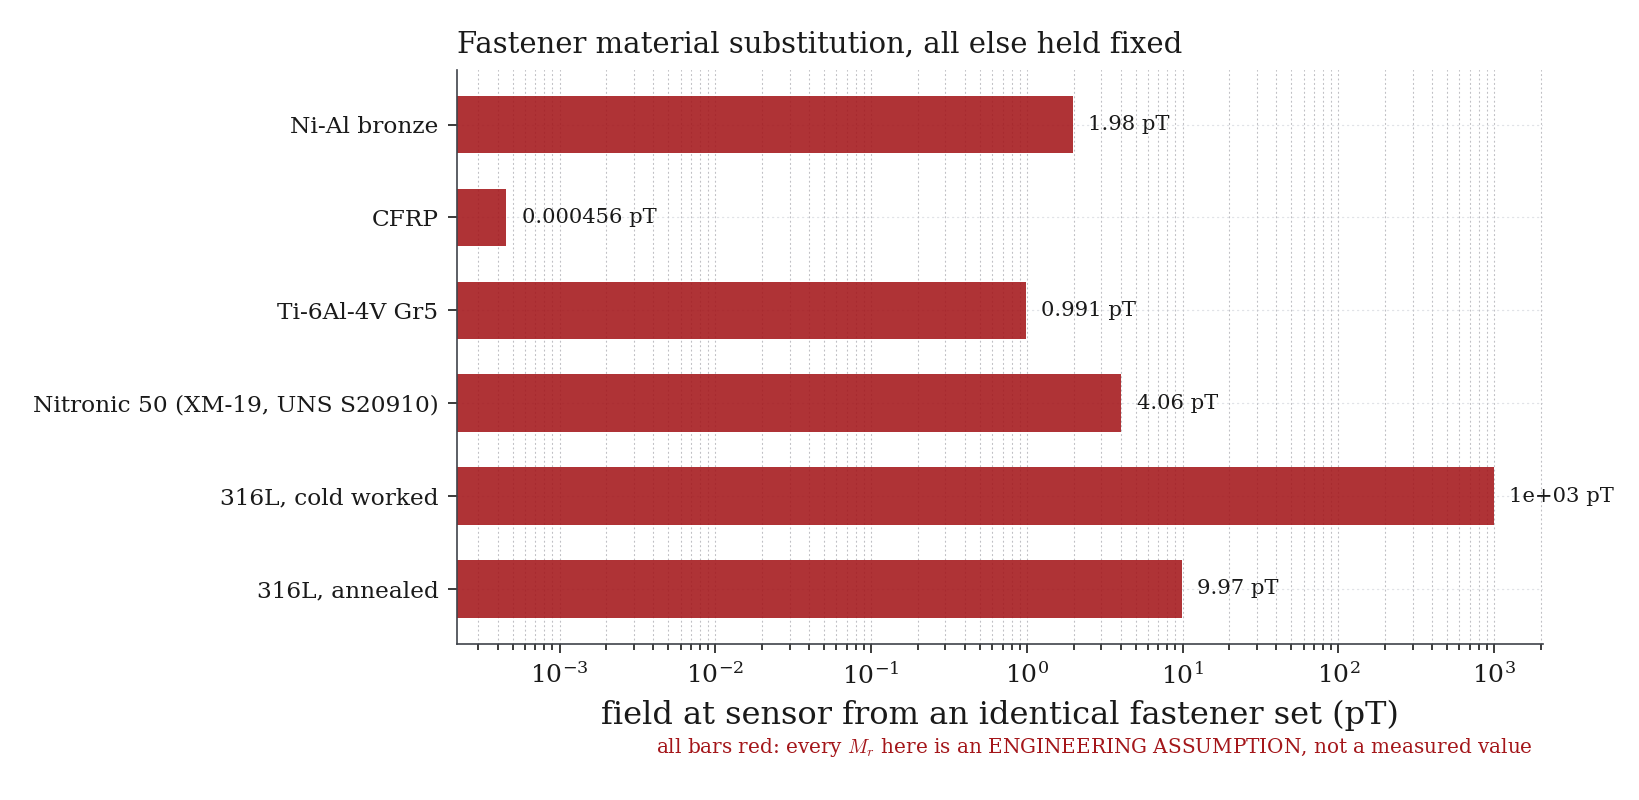
\includegraphics[width=0.72\linewidth]{outputs_materials/fig_mat_fastener.png}
\caption{Field at the sensor from an identical fastener set in each candidate
material\sig. All bars are drawn in the assumption colour because the remanence
driving each is assumed, not measured.}\label{fig:fastener}
\end{figure}

The recommendation that follows is narrow and actionable: specify
\textbf{Nitronic~50 for fasteners} rather than 316L, on the documented grounds
that it does not form martensite on cold work \cite{bssa,electralloy50}, and
prefer CFRP for non-load-bearing payload structure.

\subsection{Shielding materials and the forming penalty}
Requirement R-02 asks for $\geq94$~dB of combined suppression. Equation
\eqref{eq:req} implies $53{,}191\times$ total; against the parent study's
$100\times$ active stage the passive stage must therefore supply
$532\times$\lit.

For a single-layer cylindrical shield the amplitude response is
$T=D/(\mu_r\Delta)$ for diameter $D$ and wall thickness $\Delta$
\cite{dubbers1986}, so the shielding factor is
\begin{equation}
S=\frac{\mu_r\,\Delta}{D} .
\label{eq:shield}
\end{equation}
This is a literature closed form; the fuller cylindrical treatment is
\cite{hoburg1996} and the multi-shell case, which is \emph{not} modelled here,
is \cite{sumner1987,celozzi2008}. Evaluating Eq.~\eqref{eq:shield} with measured
permeabilities \cite{gohil2020} gives Table~\ref{tab:shield}.

\begin{table}[htbp]\centering\small
\begin{tabular}{llrrrc}
\toprule
\textbf{Condition}&\textbf{$\mu_r$}&\textbf{$D$}&\textbf{$\Delta$}&\textbf{$S$}&\textbf{Meets $532\times$?}\\
\midrule
Annealed in final form&$55{,}955$ \meas&$5$~cm&$1.0$~mm&$1119\times$&yes ($2.1\times$ margin)\\
Annealed in final form&$55{,}955$ \meas&$10$~cm&$1.0$~mm&$559\times$&marginal ($1.05\times$)\\
Foil, formed, not re-annealed&$4{,}660$ \meas&$5$~cm&$1.0$~mm&$93\times$&\textbf{no} (short $5.7\times$)\\
Foil, formed, not re-annealed&$4{,}660$ \meas&$10$~cm&$1.0$~mm&$47\times$&\textbf{no} (short $11.4\times$)\\
\bottomrule
\end{tabular}
\caption{Passive shielding from Eq.~\eqref{eq:shield}\lit, using the initial
permeabilities measured in \cite{gohil2020}. Permeabilities are measured; the
shielding factors are a closed form evaluated here, not a simulation
result.}\label{tab:shield}
\end{table}

\begin{figure}[htbp]\centering
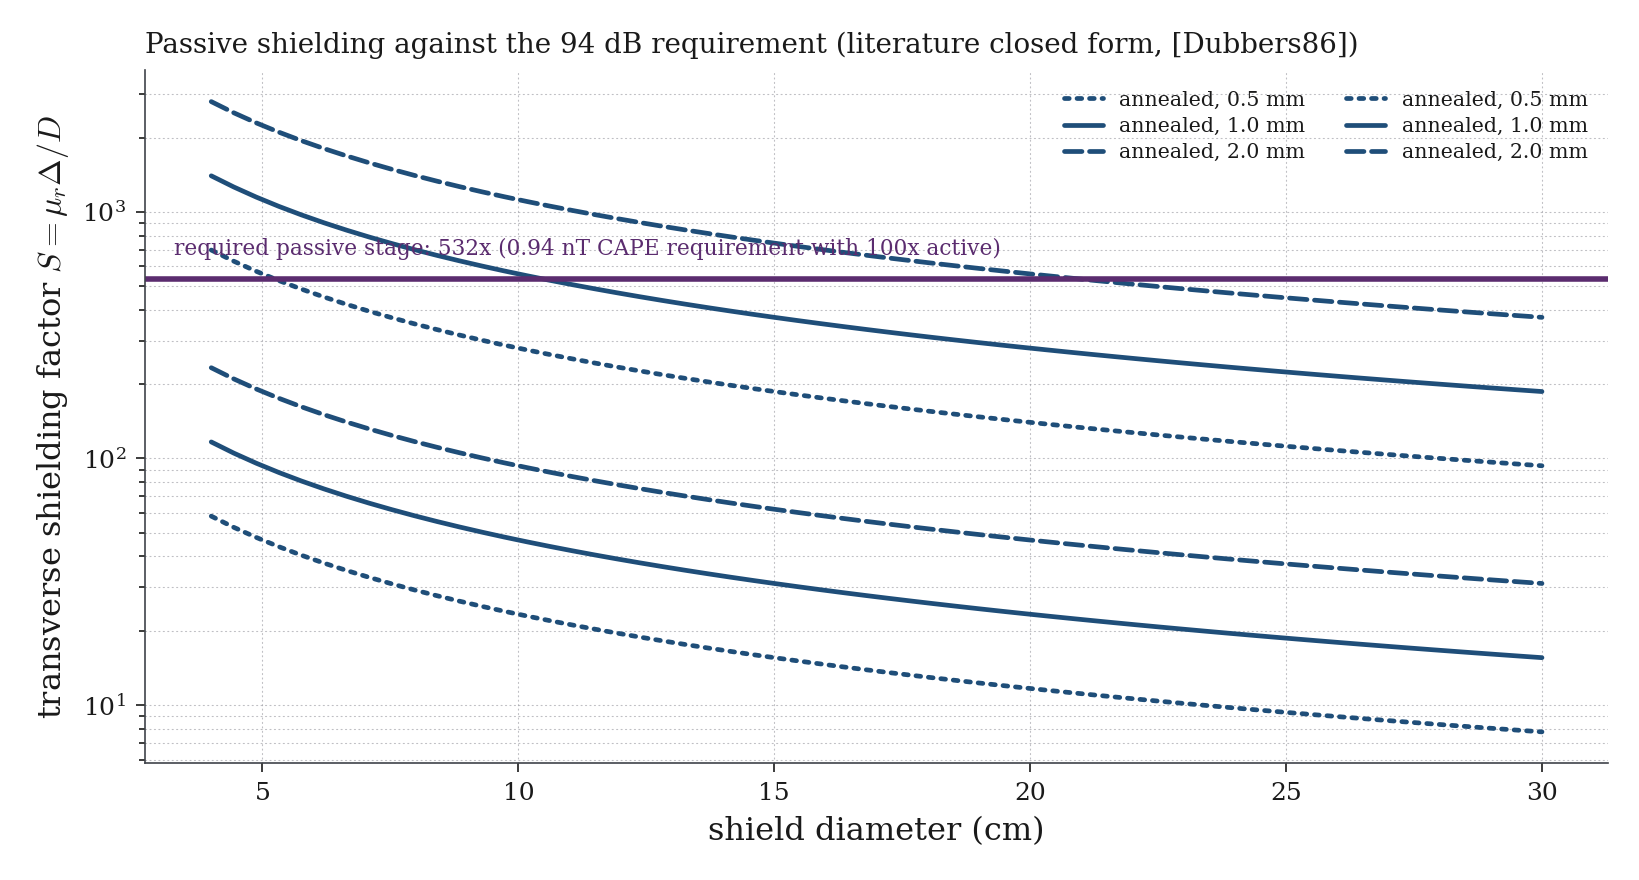
\includegraphics[width=0.70\linewidth]{outputs_materials/fig_mat_shielding.png}
\caption{Shielding factor against shield diameter for annealed and formed
mu-metal at three wall thicknesses\lit, with the $532\times$ passive requirement
marked.}\label{fig:shield}
\end{figure}

Two conclusions follow, and the second is the more important.

First, the budget \emph{closes} --- but not with margin to spare. An annealed
mu-metal shield of $5$~cm diameter and $1$~mm wall clears the requirement by a
factor of $2.1$. At $10$~cm, a more plausible envelope once coils, oven and
insulation are accommodated, the margin is $1.05$ and effectively gone. Shield
diameter is thus a first-order payload architecture parameter, not a detail.

Second, \textbf{the same alloy fails if it is formed and not re-annealed}.
\cite{gohil2020} measured $\mu_i=55{,}955\pm7$ for an annealed cylinder but only
$3{,}670$, $3{,}602$ and $4{,}660$ for three shields rolled from foil and not
re-annealed, attributing the loss to deformation during forming\meas. Recovery
requires annealing above $1000^\circ$C, which cannot be applied to an assembled
payload. For a vehicle-mounted instrument that must survive launch, recovery,
vibration and pressure cycling this is a live risk: a shield deformed in service
does not fail loudly, it quietly stops shielding, and the parent study notes that
loss of SERF lock does not degrade gracefully.

\subsection{Thermal materials}
Requirement R-07 asks for $150$--$200^\circ$C at $\pm5$~mK using non-magnetic
heating \cite{fang2015}. Silica aerogel is the preferred insulation on two
independent grounds: its thermal conductivity is roughly half that of still air,
which is what makes the budget tractable in cold seawater, and it is an
electrical insulator, so unlike a metallic jacket it can support neither eddy
currents nor Johnson noise near the cell \cite{lee2008}. Both figures are
assumptions in the present schema\assm.

Two incompatibilities are worth recording. The epoxy matrix of CFRP has a service
limit at the \emph{bottom} of the cell operating range, so CFRP must not contact
the cell oven\assm. And nickel-aluminium bronze, the traditional non-magnetic
marine fitting alloy, has the highest conductivity of any candidate here
($4.3\times10^{6}$~S/m\assm) and is therefore the material most likely to become
a Johnson-noise problem adjacent to the cell --- a term this work does not yet
compute, as Section~8 states.

\section{Integration Architecture: A Geometry-Derived Rejection Limit}
\subsection{Two rejection regimes}
A two-cell gradiometer forms $(B_1-B_2)/L$. How well it rejects an interferer
depends on where that interferer is, and the two regimes differ by orders of
magnitude.

For a \textbf{distant, uniform} source the field is equal at both cells to high
accuracy, so the differential output is set purely by how well the channels are
matched. With the $\leq0.1\%$ gain and axis matching of R-09 the rejection is
$1/10^{-3}=60$~dB. \emph{This is the regime the widely quoted figure describes,
it applies to the Earth's field, and nothing in this report disputes it.}

For a \textbf{near-field} source --- a thruster or battery metres from the
baseline --- the field genuinely differs between the cells. That difference is a
real differential signal, not a mismatch artefact, and no amount of channel
matching removes it. For a dipole at standoff $d$ with baseline $L$ along the
same axis, $B\propto r^{-3}$ gives a differential-to-common ratio of
approximately $3L/d$, hence
\begin{equation}
\mathrm{CMRR}\;\approx\;\frac{d}{3L} .
\label{eq:cmrr}
\end{equation}

\subsection{Model and calibration}
The vehicle is represented as a superposition of point-dipole sources at
body-frame positions, evaluated with the parent study's already-verified dipole
and gradient-tensor code (its tests V-01 to V-03 pass at $10^{-12}$,
$7.4\times10^{-10}$ and $6.4\times10^{-16}$). Structural components take their
moments from the material schema; motors and battery packs instead carry an
explicit assumed moment, because a brushless motor's magnetic circuit closes its
flux through the stator so its net external moment is far below the sum of its
magnets', and a battery's moment is dominated by DC current loops rather than by
material susceptibility. Deriving those from $M_r V$ would be a fabricated
calculation, and the schema records which route each component used.

The reference REMUS-class layout is calibrated so that its total field at the
baseline centre reproduces the $246.90\nT$ raw UUV interference measured before
compensation \cite{oehler2024} --- the only measured anchor available.
Verification test M-07 asserts this to a relative error below $10^{-9}$\sig. The
calibration constrains the \emph{total} only; the component split remains an
assumption.

\subsection{Result}
Table~\ref{tab:cmrr} and Figure~\ref{fig:cmrr} give the derived rejection.
Verification test M-02 confirms the full vector superposition converges to
Eq.~\eqref{eq:cmrr} in the far field, and M-03 that rejection increases
monotonically with standoff, which is the quantitative content of R-13.

\begin{table}[htbp]\centering\small
\begin{tabular}{rrrrl}
\toprule
\textbf{Standoff}&\textbf{Derived CMRR}&\textbf{Shortfall vs $60$~dB}&\textbf{$R_{50}$}&\textbf{Binding mechanism}\\
\midrule
$1$~m&$1.9$~dB&$58.1$~dB&$13.89$~m&geometry\\
$2$~m&$5.5$~dB&$54.5$~dB&$15.07$~m&geometry\\
$3$~m&$8.1$~dB&$51.9$~dB&$15.88$~m&geometry\\
$5$~m&$11.7$~dB&$48.3$~dB&$17.16$~m&geometry\\
$10$~m&$17.1$~dB&$42.9$~dB&$19.90$~m&geometry\\
\midrule
assumed&$60.0$~dB&---&$66.75$~m&matching\\
\bottomrule
\end{tabular}
\caption{Derived common-mode rejection and the resulting detection range against
a naval-mine-class target\sig, baseline $0.5$~m. Geometry binds at every
realistic standoff. The assumed row reproduces the parent study's published
$R_{50}$ of $67.6$~m to within its documented seed spread.}\label{tab:cmrr}
\end{table}

\begin{figure}[htbp]\centering
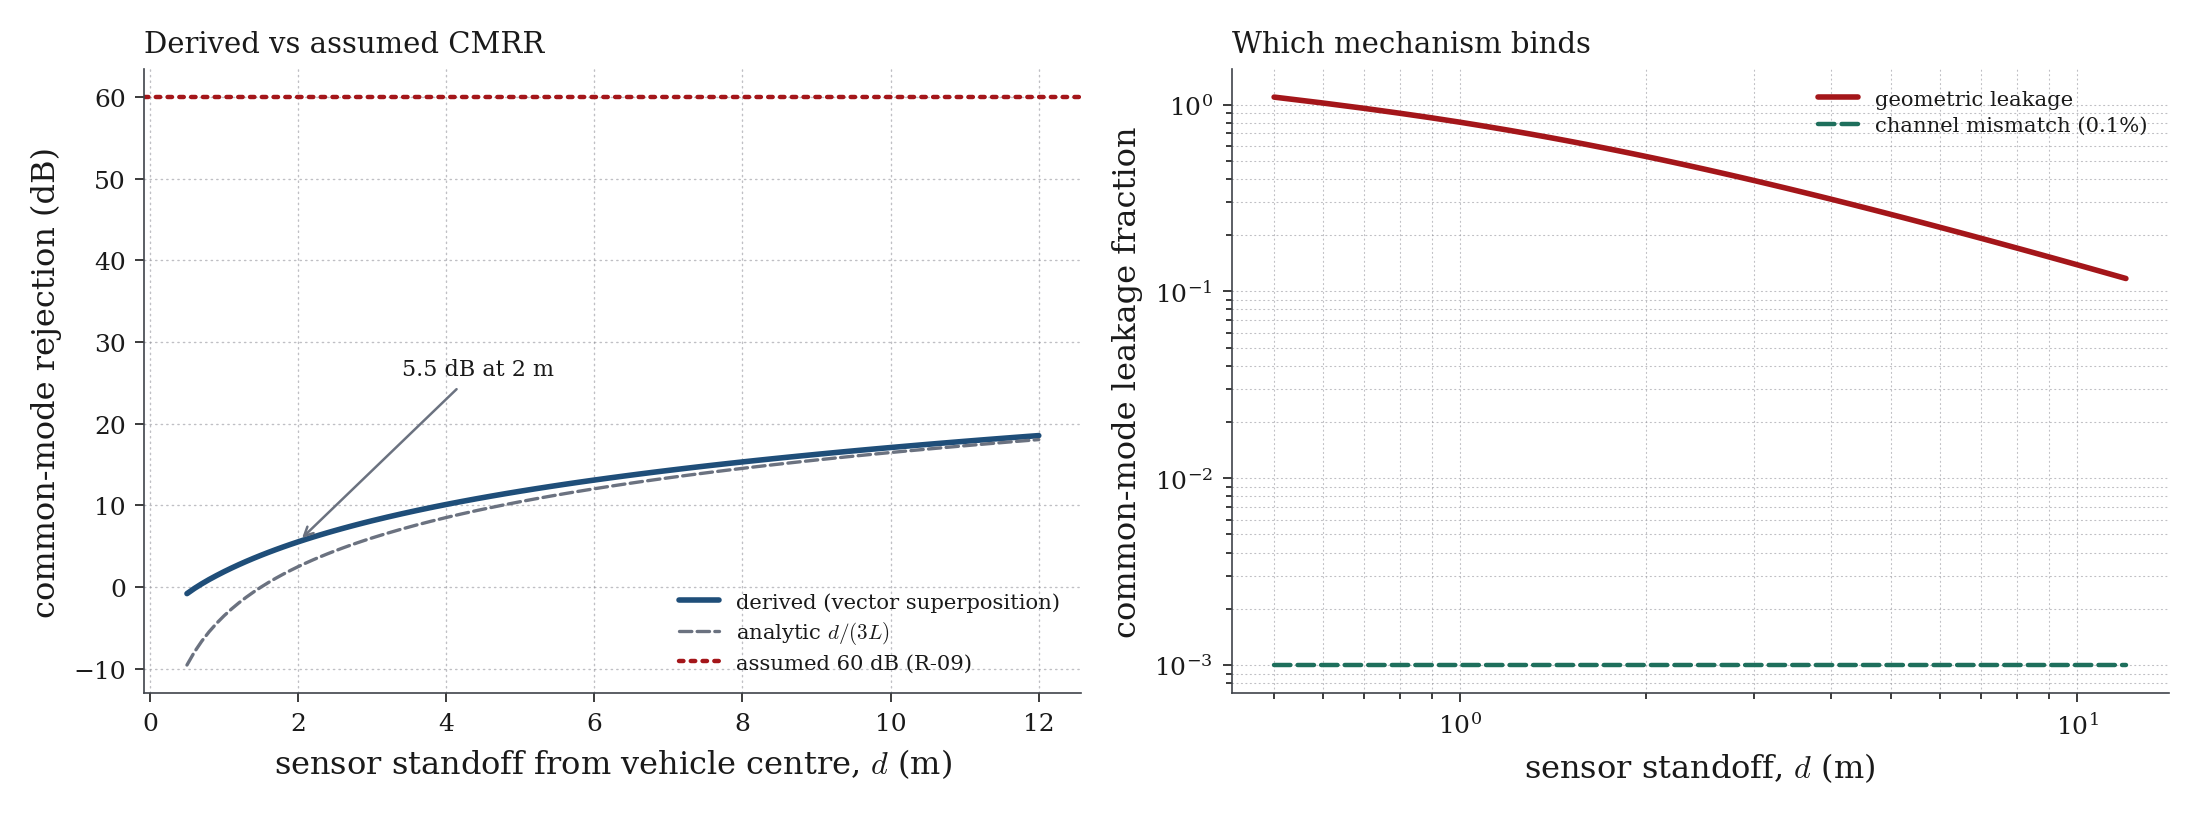
\includegraphics[width=0.94\linewidth]{outputs_materials/fig_mat_cmrr_standoff.png}
\caption{Left: derived rejection against standoff\sig, with the analytic
$d/(3L)$ estimate and the assumed $60$~dB. Right: the two leakage mechanisms.
Geometric leakage exceeds channel mismatch by two to three orders of magnitude
throughout the plausible range.}\label{fig:cmrr}
\end{figure}

\subsection{Detection consequence}
The derived rejection was propagated through the parent study's \emph{unmodified}
Monte Carlo detection chain, with identical range bounds, trial count and seed;
the only argument changed between rows is the rejection ratio, so the difference
is attributable to it alone. Detection range falls to $21$--$30\%$ of the
figure obtained under the assumed rejection (Figure~\ref{fig:detection}).

\begin{figure}[htbp]\centering
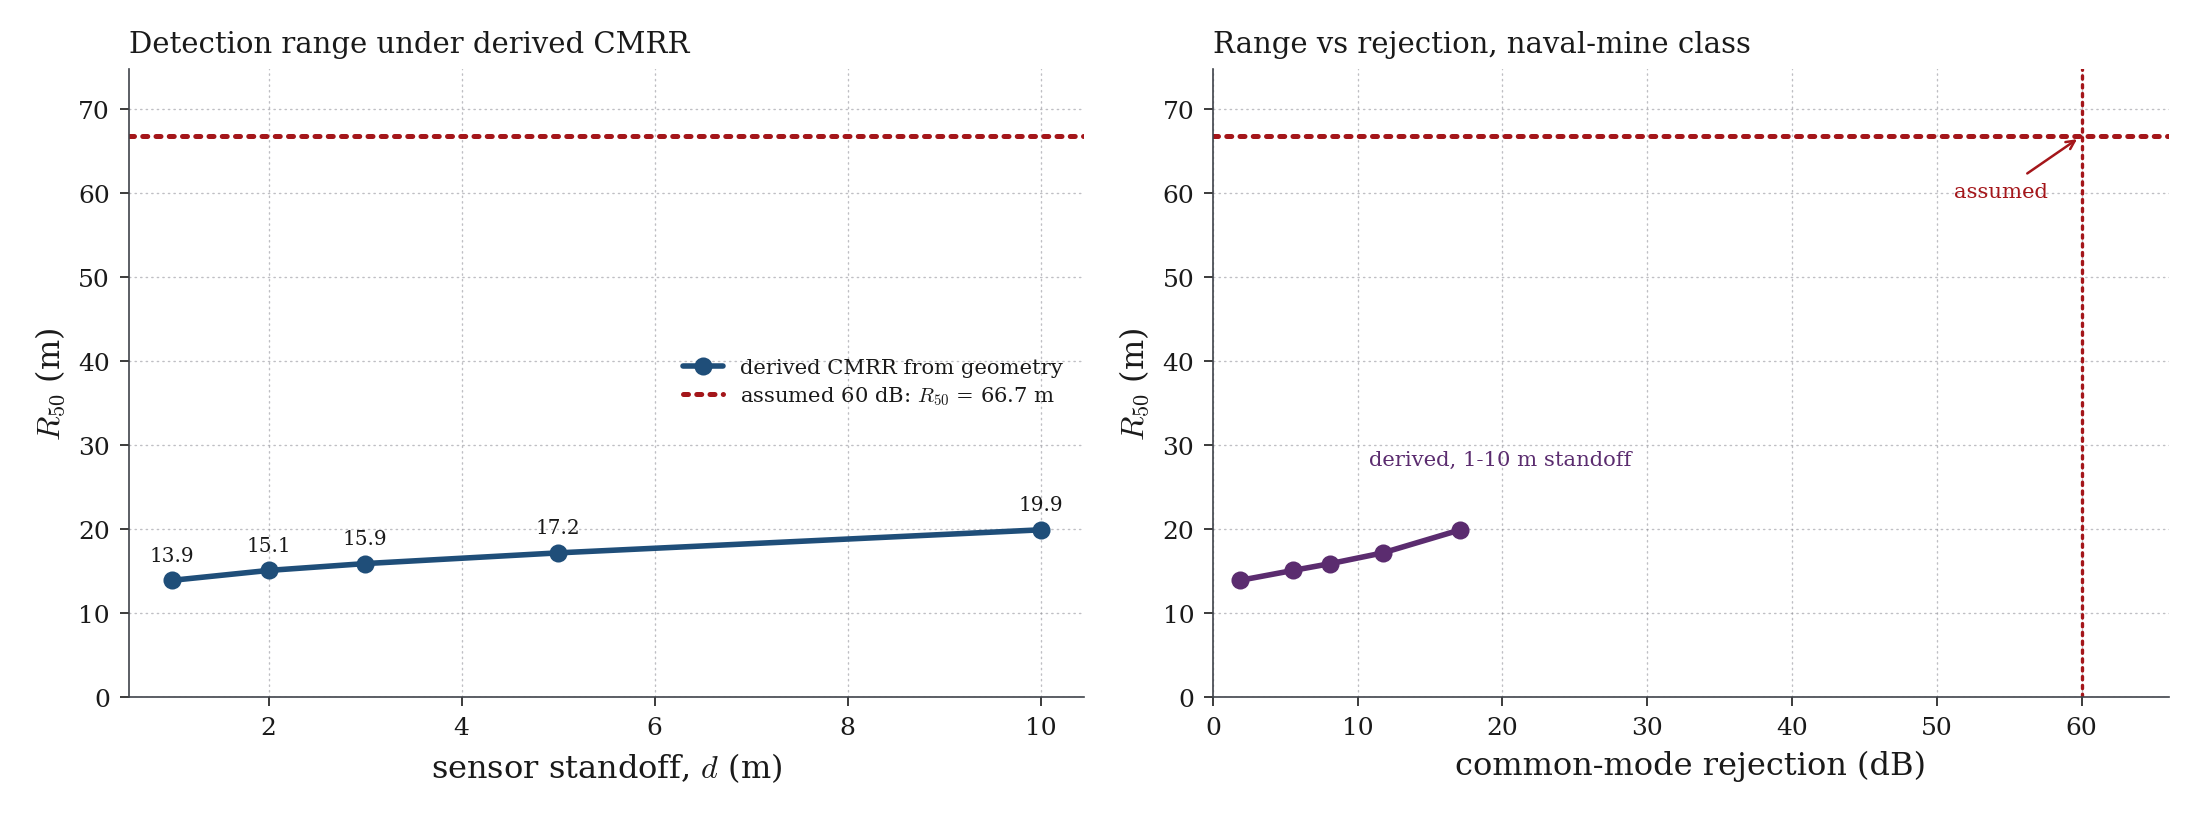
\includegraphics[width=0.94\linewidth]{outputs_materials/fig_mat_detection.png}
\caption{Detection range under the derived rejection\sig, against the
assumed-rejection baseline of $66.75$~m.}\label{fig:detection}
\end{figure}

\subsection{Why standoff cannot fix this}
Equation~\eqref{eq:cmrr} is linear in $d$ while the absolute field falls as
$d^{-3}$, and the difference matters. Reaching $60$~dB of \emph{rejection} by
displacement alone would require $d=3L/10^{-3}=1500$~m at a $0.5$~m baseline.
A boom cannot deliver that; neither can a tow.

What displacement \emph{does} deliver is a reduction in the absolute clutter
field, eightfold per doubling. That is precisely why R-13 remains sound advice
and why the Girona~500's $2$--$3$~m standoff \cite{seidel2023} is well judged.
But it means the two must not be conflated: \textbf{standoff reduces how much
clutter there is; it does not much improve the gradiometer's ability to reject
what remains.}

The design conclusion is that platform interference must be attacked at the
source, in absolute terms, by material selection and current-loop control at
build time --- which is the subject of Section~4 and the thesis of this report.
Gradiometry and compensation are second lines of defence, not substitutes.

\section{Integration Architecture and TRL Path}
\subsection{Architecture recommendations}
\begin{table}[H]\centering\small
\begin{tabular}{p{1.0cm}p{3.2cm}p{7.2cm}p{4.0cm}}
\toprule
\textbf{Req}&\textbf{Subsystem}&\textbf{Recommendation}&\textbf{Basis}\\
\midrule
I-01&Sensor mounting&Rigid boom, not tow cable; baseline held by a structure that cannot flex between cells&\cite{seidel23sheet}; R-09 matching\\
I-02&Standoff&$2$--$3$~m forward of the hull, away from thrusters; treat as clutter reduction, not rejection&\cite{seidel2023}; Eq.~\eqref{eq:cmrr}\\
I-03&Fasteners&Nitronic 50 (XM-19); do not accept 316L on a non-magnetic certification alone&\cite{bssa,electralloy50}; Table~\ref{tab:fastener}\\
I-04&Payload structure&CFRP where non-load-bearing; Ti-6Al-4V where load-bearing&Table~\ref{tab:fastener}\\
I-05&Shield&Mu-metal annealed \emph{in final form}; diameter is a first-order parameter&Table~\ref{tab:shield}; \cite{gohil2020}\\
I-06&Shield handling&Treat post-anneal deformation as a functional failure; no field re-forming&\cite{gohil2020}\\
I-07&Cell insulation&Silica aerogel; electrically insulating, so it adds no Johnson noise&\cite{lee2008}; R-07\\
I-08&Near-cell metals&Avoid high-conductivity alloys (Ni-Al bronze) adjacent to the cell&\cite{lee2008}\\
I-09&Rejection budget&Do not budget $60$~dB against platform sources; use the derived value for the actual geometry&Table~\ref{tab:cmrr}\\
\bottomrule
\end{tabular}
\caption{Integration recommendations. I-09 supersedes the use of a uniform-field
rejection figure for near-field platform clutter.}\label{tab:integ}
\end{table}

\subsection{TRL position and gating experiments}
The parent study places the integrated concept at TRL~3--4 with integration risk
concentrated in the nulling servo. This work does not advance that position ---
it sharpens where the remaining risk sits, and adds a second concentration of
risk in whole-vehicle magnetic cleanliness. Both are testable cheaply relative
to development, and the ordering below is by information gained per unit cost.

\begin{enumerate}[leftmargin=1.5em]
\item \textbf{Measure $M_r$ of worked fasteners.} The single highest-value
measurement in this report. Table~\ref{tab:fastener} is driven entirely by
assumed remanence values; a bench measurement of representative 316L and
Nitronic~50 fasteners, before and after heading and thread rolling, would replace
the largest assumption in the model with data. Cost: a fluxgate, a turntable, and
a box of bolts.
\item \textbf{Measure formed-shield permeability.} Verify the
\cite{gohil2020} forming penalty on the actual shield geometry and forming
process proposed, since Table~\ref{tab:shield} turns on it.
\item \textbf{Bench-test rigid boom versus tow cable} for gradiometer baseline
stability, closing the gap identified in Section~3.2.
\item \textbf{Measure the candidate vehicle's magnetic signature} versus
distance, replacing the single-anchor calibration of Section~5.2 with a
component-resolved map. The parent study's Recommendation~7 already asks for
this; the present model makes its output directly consumable.
\item \textbf{Implement the eddy-current and Johnson-noise term} so the
conductivity column of the schema drives a result, as discussed in Section~8.
\end{enumerate}

\section{What Changed and What Did Not}
Because this report revises a quantity used in a published study, it is worth
being explicit about the boundaries of the claim.

\textbf{Unchanged.} The CAPE requirement of Eq.~\eqref{eq:req} and the $94$~dB
figure; the clutter-limited finding; the sensor noise floor and its five-order
margin; all twenty-seven verification, validation and stress results; every
published figure, which remains byte-identical. Nothing in the parent study has
been recomputed or restated incorrectly.

\textbf{Refined.} The interpretation of the $60$~dB rejection figure. It remains
correct for uniform fields, which is the regime R-09's matching specification
addresses. What this work shows is that it does not transfer to near-field
platform sources, and that the parent study's own X-07 discussion --- which notes
that vehicle sources ``lie metres from the baseline, their field has a genuine
gradient across it and cancellation is necessarily imperfect'' --- anticipates
exactly this and is here made quantitative.

\textbf{New.} A material property layer that did not previously exist; a
geometry-derived rejection ratio; the forming-penalty result for shield material;
and the remanence-versus-susceptibility distinction as a build-time constraint.

\textbf{Not claimed.} That the parent study's detection ranges are wrong. They
are correct given their stated assumption. The derived ranges in
Table~\ref{tab:cmrr} rest on a vehicle model whose component split is assumed and
whose calibration has a single anchor, and they should be read as showing the
\emph{sensitivity} of the published figures to a parameter that was previously
free --- not as a replacement capability estimate.

\section{Limitations}
\begin{enumerate}[leftmargin=1.5em]
\item \textbf{$84\%$ of schema property values are assumptions.} The most
consequential is the remanence of cold-worked 316L, which drives
Table~\ref{tab:fastener} and has no measured basis. The ranking of materials is
robust because it follows from whether a ferromagnetic phase can form; the
magnitudes are not.
\item \textbf{Single-anchor calibration.} The vehicle model matches one measured
number \cite{oehler2024}. A model with a correct total and an incorrect spatial
distribution would produce a plausible common-mode field and an incorrect
gradient, and nothing here excludes that.
\item \textbf{No eddy-current or Johnson-noise term.} Conductivity is carried in
the schema and reported but drives no result. The parent study cites
\cite{lee2008} for a shield noise floor that is likewise asserted rather than
computed; closing this remains open in both.
\item \textbf{Point-dipole sources.} Valid beyond roughly one body length of each
source; comfortable at a $2$~m standoff from a $0.1$~m motor, marginal for the
pressure housing treated as a lumped source at the vehicle centre.
\item \textbf{Single-layer shielding only.} Eq.~\eqref{eq:shield} does not cover
the multi-shell configurations \cite{sumner1987} that a real payload would
likely use, and which would ease the diameter constraint of
Table~\ref{tab:shield}.
\item \textbf{Anisotropy discarded.} CFRP conductivity spans roughly seven orders
of magnitude between in-plane and through-thickness; a scalar is a poor
description and is retained only because no conductivity-driven physics consumes
it yet.
\item \textbf{No hydrodynamic simulation.} Section~3 is literature only, by
scope. The two computed rows in Table~\ref{tab:attitude} use measured attitude
figures as inputs to an existing validated model; they are not a hydrodynamic
prediction.
\end{enumerate}

\section{Conclusion}
The parent study concluded that a ruggedised SERF MEMS magnetometer is a
physically credible AUV MAD payload whose feasibility is governed by ambient
field control and platform magnetic cleanliness rather than by sensor
sensitivity. This report accepts that conclusion and examines the second of those
two constraints in the terms it actually presents itself: structure, materials,
and where things are placed.

Three findings result. Gradiometric rejection of platform sources is limited by
geometry rather than by channel matching, giving $5.5$~dB at a realistic $2$~m
standoff against the $60$~dB appropriate to a uniform field, and displacement
cannot close that gap because rejection improves only linearly in standoff.
Magnetic cleanliness is dominated by remanence, which survives ambient-field
nulling and is therefore fixed at build time, making fastener metallurgy a
first-order design parameter rather than a procurement detail. And the passive
shield closes the $94$~dB budget only when annealed in its final form, since
forming without re-annealing costs an order of magnitude of permeability that
cannot be recovered on an assembled payload.

The unifying conclusion is that platform interference must be attacked at the
source. Gradiometry, compensation and field control are all second lines of
defence, and none of them substitutes for a vehicle that is quiet to begin with.
The highest-value next step is inexpensive: measure the remanence of worked
fasteners, and replace the largest assumption in this report with a number.

\begin{thebibliography}{99}\small
\bibitem{srreport} \emph{Feasibility of a Ruggedised SERF MEMS Vapour-Cell
Magnetometer for Magnetic Anomaly Detection from an Autonomous Underwater
Vehicle}, Scientific Report, companion document (2026). Source of the CAPE
requirement, the clutter-limited finding, and the verification, validation and
stress suites referenced throughout.

\bibitem{allred2002} J.~C.~Allred, R.~N.~Lyman, T.~W.~Kornack, and M.~V.~Romalis,
``High-sensitivity atomic magnetometer unaffected by spin-exchange relaxation,''
\emph{Phys. Rev. Lett.} \textbf{89}(13), 130801 (2002).
DOI:10.1103/PhysRevLett.89.130801.

\bibitem{griffith2010} W.~C.~Griffith, S.~Knappe, and J.~Kitching, ``Femtotesla
atomic magnetometry in a microfabricated vapor cell,'' \emph{Opt. Express}
\textbf{18}(26), 27167--27172 (2010). DOI:10.1364/OE.18.027167.

\bibitem{borna2022} A.~Borna, J.~Iivanainen, T.~R.~Carter, J.~McKay, S.~Taulu,
J.~Stephen, and P.~D.~D.~Schwindt, ``Cross-axis projection error in optically
pumped magnetometers and its implication for magnetoencephalography systems,''
\emph{NeuroImage} \textbf{247}, 118818 (2022).
DOI:10.1016/j.neuroimage.2021.118818.

\bibitem{oehler2024} M.~Oehler \emph{et al.}, ``Processing of unmanned underwater
vehicle vector magnetometer data,'' \emph{Geophysical Prospecting} \textbf{72}
(2024). DOI:10.1111/1365-2478.13556. Source of the $246.90\nT$ raw and
$2.23\nT$ post-compensation UUV interference benchmark.

\bibitem{seidel2023} M.~Seidel, T.~Frey, and J.~Greinert, ``Underwater UXO
detection using magnetometry on hovering AUVs,'' \emph{Journal of Field
Robotics} \textbf{40}, 848--861 (2023). DOI:10.1002/rob.22159.

\bibitem{seidel23sheet} CONMAR project / GEOMAR Helmholtz Centre for Ocean
Research Kiel, ``AUV-based Magnetometry,'' project product sheet (accessed
2026). Girona~500 with four SENSYS FGM3D/100~UW~II three-axis fluxgates at
$200$~Hz; states that the rigid construction holding the magnetometers
suppresses spatial errors that towed systems usually produce.

\bibitem{waveglider2025} ``An Affordable Wave Glider-Based Magnetometry System
for Marine Magnetic Measurement,'' \emph{J. Mar. Sci. Eng.} \textbf{13}(11),
2089 (2025). DOI:10.3390/jmse13112089. Twin-body towed configuration with an
S-shaped cable; measured towed-body pitch within $\pm5^\circ$ and roll within
$\pm1^\circ$ at $0.56$~m/s.

\bibitem{gohil2020} C.~Gohil, P.~N.~Burrows, N.~Blaskovic~Kraljevic, D.~Schulte,
and B.~Heilig, ``Measurements of sub-nT dynamic magnetic field shielding with
soft iron and mu-metal for use in linear colliders,'' arXiv:2009.01519v2 (2020).
Measured $\mu_i=55{,}955\pm7$ for annealed mu-metal against $3{,}670$, $3{,}602$
and $4{,}660$ for formed, un-re-annealed foil shields.

\bibitem{dubbers1986} D.~Dubbers, ``Simple formula for multiple mu-metal
shields,'' \emph{Nucl. Instrum. Meth. A} \textbf{243}, 511--517 (1986). Source
of the single-layer shielding factor of Eq.~\eqref{eq:shield}.

\bibitem{sumner1987} T.~J.~Sumner, J.~M.~Pendlebury, and K.~Smith, ``Convectional
magnetic shielding,'' \emph{J. Phys. D: Appl. Phys.} \textbf{20}, 1095 (1987).

\bibitem{hoburg1996} J.~F.~Hoburg, ``Principles of quasistatic magnetic
shielding with cylindrical and spherical shields,'' \emph{IEEE Trans.
Electromagn. Compat.} \textbf{38}, 93--103 (1996).

\bibitem{celozzi2008} S.~Celozzi, R.~Araneo, and G.~Lovat, \emph{Electromagnetic
Shielding}, John Wiley \& Sons (2008).

\bibitem{assda} Australian Stainless Steel Development Association, Technical
FAQ 3, ``Magnetic Effects of Stainless Steels.'' Annealed 316/317L DC
permeability $1.003$--$1.005$ at $200$~oersteds.

\bibitem{bssa} British Stainless Steel Association, ``Effect of cold work and
heat treatment on the magnetic permeability of austenitic stainless steels.''
Grades of high austenite stability retain low permeability in both annealed and
cold-worked conditions.

\bibitem{electralloy50} Electralloy / G.O. Carlson, NITRONIC 50 (XM-19,
UNS S20910) product data sheet. Typical annealed magnetic permeability $1.004$
at $50$, $100$ and $200$ oersteds.

\bibitem{matwebti64} MatWeb material data sheet, ``Titanium Ti-6Al-4V (Grade 5),
Annealed.'' Density, tensile and thermal properties.

\bibitem{lee2008} S.-K.~Lee and M.~V.~Romalis, ``Calculation of magnetic field
noise from high-permeability magnetic shields and conducting objects with simple
geometry,'' \emph{J. Appl. Phys.} \textbf{103}(8), 084904 (2008).

\bibitem{fang2015} J.~Fang, R.~Li, L.~Duan, Y.~Chen, and W.~Quan, ``Study of the
operation temperature in the spin-exchange relaxation free magnetometer,''
\emph{Rev. Sci. Instrum.} \textbf{86}, 073116 (2015).

\bibitem{jackson1998} J.~D.~Jackson, \emph{Classical Electrodynamics}, 3rd ed.,
Wiley, New York (1998), Ch.~5.
\end{thebibliography}

\vfill
\band
\end{document}
